% TODO: be careful about uniform classes, should be explicit and mentioned
% TODO: add paragraph on kernelization (and other techniques?)
% TODO: Make sure to integrate vertex cover param./example/reductions in the report

\documentclass[a4paper,11pt,notitlepage]{report}

\usepackage{amsthm}
\usepackage{complexity}
\usepackage{amsfonts}
\usepackage[british,english]{babel}
\usepackage[T1]{fontenc}
\usepackage[utf8x]{inputenc}
\usepackage{listings, babel}
\usepackage{graphicx}
\lstset{breaklines=true,basicstyle=\ttfamily}
\usepackage[margin=2cm]{geometry}

\theoremstyle{plain}
\newtheorem{thm}{Theorem}[chapter] % reset theorem numbering for each chapter

\theoremstyle{definition}
\newtheorem{defn}[thm]{Definition} % definition numbers are dependent on theorem numbers
\newtheorem{exmp}[thm]{Example} % same for example numbers

\newcommand{\PARANP}{\ComplexityFont{paraNP}}

\selectlanguage{english}
\title{report title}
\author{David Nilsson, davnils@kth.se \\ Advanced Individual Course In Computer Science}

\begin{document}

\maketitle
\clearpage

\abstract{TODO}
\selectlanguage{english}

\tableofcontents

\chapter{Project Overview}
This is an overview of this project, including goals and how the report is outlined.

\section{Purpose}
The purpose of this project is divided into two parts.
TODO the first part
TODO the second part

\section{Method}
TODO: Describe how this report fits into the bigger picture, what else has been
done, and what the report contains.

\chapter{Parameterized Complexity Theory}
TODO: Brief intro to this chapter

\section{Motivation}
In classical complexity theory we are given a very general view of computation.
The asymptotic time and space complexity of problems is given as functions over the number of bits in the input.
This results in the classification of many problems as \NP-hard (e.g. vertex cover, independent set), which is typically interpreted as the problem being difficult to solve.
Does exluding polynomial time algorithms for problems in general make them infeasible in practice?
For certain problems this might certainly be true but there is no fundamental reason to which this would hold in general.
Many problems have special cases that are easy to solve or approximation algorithms that are capable of finding decent solutions within polynomial time.
For example there might exist a polynomial time algorithm solving all cases when an aspect of the problem is considered constant, e.g. the number of vertices in a vertex cover.

Parameterized complexity theory aims to provide a theoretical foundation for asymptotic analysis on a more fine-grained scale.
This is achieved by not only considering inputs as a binary string but placing it into a context of the problem being solved.
All of this is achieved while still maintaining classical complexity classes and focusing on existing results.
This alternative view of complexity theory also forms natural ties with approximation algorithms, something which is studied in REF.

\section{Parameterized decision problems}
The first step in developing a more fine-grained theory is to describe how problems are expressed.
In addition to strings in the language $L$ to be decided, the following is also needed:

\begin{defn}
A \emph{parameterization} is a polynomial time computable function $k : \Sigma^* \rightarrow \mathbb{N}$
\end{defn}

A parameterized decision problem is given on the format: $(L, k)$ where $L \subseteq \Sigma^*$ and $k$ is a parameterization of $L$.
The following is a common parameterization of vertex cover, known as $p-VERTEX-COVER$:
\begin{itemize}
\item Input: Graph $G$, number of vertices in cover $s$
\item Parameterization: $k((G, s)) = s$.
\item Problem: Does $G$ have a vertex cover of size $\leq s$?.
\end{itemize}

In classical complexity theory, reductions are given between problems as polynomial time computable mappings between strings in the languages.
Naturally this notion does not extend trivially to parameterized problems since the parameterization must be handled as well.
This results in the following:

\begin{defn}
A reduction $R$ mapping strings between the two parameterized languages $(L, k)$ and $(L', k')$ satisfies:
\begin{itemize}
\item the reduction preserves membership, i.e $x \in L \Leftrightarrow R(x) \in L'$
\item $R(x)$ is computable in time $f(k(x)) |x|^{O(1)}$ for any $x \in L$, where $f$ is a computable function
\item there is some computable function $f(x) : \mathbb{N} \rightarrow \mathbb{N}$ s.t. $\forall x \in \Sigma^* : k'(x) < f(k(x))$
\end{itemize}
\end{defn}

Typically such a reduction is written as $L <^{fpt} L'$.
The specific runtime bound is common within parameterized complexity and will later play a crucial part when defining fixed parameter tractability.

The second constraint ensures that certain reductions are rejected as invalid reductions.
An example of this is considering vertex cover, using the parameterization in TODO, and extending this result to other graph problems.
Independent set is commonly related to vertex cover as having the size $|G| - |S|$ for a graph $G$ with vertex cover $S$ (TODO REF).
Does this imply that the decision version of independent set reduces to vertex cover under parameterized reductions, and hence also transferring hardness?
%TODO: complete argument (pro-tip: it doesn't hold!)

Furthermore, it is of interest to study if problems remain within some given set of languages when applied to some reduction $R$.

\begin{defn}
The \emph{closure} of a set $C$ of languages is defined as $\left[ C \right] = \left\{ L' : L \in C : L <^{fpt} L'\right\}$.
\end{defn}

\begin{defn}
%TODO: Verify this statement.
A set $C$ of languages is \emph{closed} if $\left[ C \right] = C$.
\end{defn}

\begin{defn}
The $n$'th slice of a parameterized problem $(L, k)$ is $\left\{ x \in L : k(x) = n \right\}$.
\end{defn}

An example of slices is \lang{3-COLORABILITY}, which is the language formed by the slice where $n = 3$ when using the standard parameterization \lang{p-COLORABILITY}.
Slices are used later on when relating parameterized complexity classes to classical ones but also when discussing hardness results.

\section{Fixed parameter tractability}
Given the formalized notion of parameterized languages it is of interest to determine relative hardness and form a natural class hierarchy.
In classical complexity we have the notions of $\P$, $\NP$, and many others, but these two capture the essential relative difficuly.

The first step is to define allowed runtime of problems considered being tractable.

\begin{defn}
A \emph{fpt-algorithm} $A(x, k)$ runs at most $f(k(x)) |x|^{O(1)}$ steps, for some computable function $f$.
\end{defn}

This definition aims to decide which problems are feasible when solving instances having the parameterization remain constant.
In practice this might correspond to checking if some graph property applies to graphs of different sizes, and having a fpt-algorithm
would correspond to reasonable scaling in running times.
Based on this definition we have a class of tractable problems:

\begin{defn}
%TODO: Verify this statement.
The class $\FPT$ consists of all languages decided by some fpt-algorithm and is closed w.r.t fpt-reductions.
\end{defn}

As an example of this we have the following:
\begin{thm}
$\textsc{p-VERTEX-COVER} \in \FPT$
\end{thm}

Proof: the following algorithm decides if $G$ has a vertex cover of size at most $k$ in time $O(2^k |E(G)|)$.
\begin{verbatim}
has-vertex-cover(E, k):
  if E = {}:
    return true
  if k == 0:
    return false

  pick some {v_1, v_2} in E
  
  E' = {}, E'' = {}
  for e in E
    if v_1 not in e:
      E' = union(E', e)
    if v_2 not in e:
      E'' = union(E'', e)

  if has-vertex-cover(E', k-1) or has-vertex-cover(E'', k-1)
    return true

  return false

\end{verbatim}

This algorithm can be seen as a binary tree of height $k$ where each node performs a linear amount of work (in the number of edges), reaching the target runtime.
It is based on the observation that deciding if a vertex cover of size $k$ exists can be expressed as a sequence of $k$ choices.
Since a valid vertex cover must include at least one vertex for each edge, every step can consider covering either vertex of an edge, and remove all covered edges.
The algorithm succeeds only when the set of edges is empty (and has hence been covered), and will fail when edges remain and $k = 0$. \qed
\\

There is a notable connection between languages in $\FPT$ and the classical class \P:

\begin{thm}
All slices of a language in $\FPT$ are in $\P$.
\end{thm}

By the contrapositive we have there is some slice $(L, k)_{l'} \not \in \P$, it follows that $(L, k) \not \in \FPT$, assuming $\P \not = \NP$.
An example of this is the fact that \lang{3-COLORABILITY} is \NP-hard, and hence under reasonable assumptions, it follows that $\lang{p-COLORABILITY} \not \in \FPT$.

\section{Generalized classes}
%TODO: This intro can be extended, for example with a formal definition of p-CLIQUE (probably should be)
The class of fixed parameter tractable languages can be seen as examples of where effective algorithms have been found.
There are however languages outside of this class; a concrete example of this is \lang{p-CLIQUE}, which will in the next section be shown to be outside of $\FPT$ under realistic complexity-theoretic assumptions.
In the case of classical complexity theory $\P$ is typically seen as the class of tractable (non-probabalistically decidable) languages and generalizations include adding non-determinism.
A similar path is taken in parameterized complexity theory where the following class is somewhat similar to $\NP$, if $\P$ is compared to $\FPT$:

\begin{defn}
$\PARANP$ is the set of parameterized languages decided by some algorithm running at most $f(k(x)) |x|^{O(1)}$ steps on a NDTM, for some computable function $f$.
\end{defn}

Naturally it holds that $\FPT \subseteq \PARANP$ since any deterministic algorithm (with equivalent time bound) can be evaluated by the corresponding NDTM.
Similarly to $NP$-complete languages there also complete languages for $\PARANP$.
These are characterized by the fact that if $(L, k) \in \PARANP$ s.t. $\exists l : (L, k)_l \in \NPC$ then $(L, k)$ is $\PARANP$-complete (TODO: Ref flum).
It is known that $\FPT = \PARANP$ iff $\P = \NP$ (TODO: REF Flum).

Another generalization is allowing more running time in the deterministic model:

\begin{defn}
(uniform) $\XP$ consists of all parameterized languages $(L, k)$ decided by an algorithm in time
$x^{f(k(x))} + f(k(x))$, for some computable function $f$.
\end{defn}

%TODO: Maybe add argument surrounding EXPTIME DTM and the following result (should probably be done as an indenpendent arugment)?

Interestingly the containment $\FPT \subset \XP$ is proper (TODO: Ref Flum).

In conclusion we have that $\FPT \subseteq \PARANP \cap \XP$.

\section{Intermediate classes}
TODO: W[P], W-hierarchy (circuit definition), relate to existing classes

\section{Hardness results and lower bounds}
TODO: why? examples using p-CLIQUE, describe K-path result

\section{Relation to approximation}
One way of approaching \NP-hard problems is to design appriximation algorithms.
The defining property is that they are guaranteed to find a solution within some time and cost bounds.

An optimization problem $O$ is typically stated as a triplet $O = (S, cost_f(x), opt_f(x))$,
where the cost and opt functions return the optimized cost and optimum respectively for some input $x$, and $S$ is the set of all solutions.

There are different classes of approximation but a central measure of optimaliity is the following:

\begin{defn}
The approximation ratio of an optimization problem $O = (S, cost_f(x), opt_f(x))$ with respect to an input $x$ is defined as:

$\textsc{ApproxRatio}_f(x) = max \left\{ \frac{opt_f(x)}{cost_f(x)}, \frac{cost_f(x)}{opt_f(x)} \right\}$
\end{defn}

Given this we have the basic definition of an algorithms finding approximate solutions in polynomial time.

\begin{defn}
A polynomial time $\epsilon$ -approximation algorithm computes solutions for inputs $x$ in polynomial time s.t. $\textsc{ApproxRatio}_f(x) \leq 1 + \epsilon$.
\end{defn}

The first very general class captures all problems approximable in polynomial time.

\begin{defn}
An optimization problem is in $\PTAS$ (i.e. there is a polynomial time approximation scheme) if there is a $\frac{1}{\epsilon}$ -polynomial time approximation algorithm for all $\epsilon$.
\end{defn}

Hence $\PTAS$ allows running times such as $O(n^{\epsilon ^ \epsilon})$, i.e. $n$ having exponential dependencies on $\epsilon$.
The well known approximation scheme by Arora (TODO: REF) to the bounded metric TSP is in $\PTAS$, with running time $O(n(\log n)^{O(\epsilon)})$.
A more refined view restricts this property:

\begin{defn}
An optimization problem is in $\EPTAS$ (i.e. there is an efficient polynomial time approximation scheme) if there is a $\frac{1}{\epsilon}$ -polynomial time approximation algorithm with 
running time $f(\frac{1}{\epsilon}) n^{O(1)}$, for some computable function $f$.
\end{defn}

\begin{defn}
An optimization problem is in $\FPTAS$ (i.e. there is a fully polynomial time approximation scheme) if there is a $\frac{1}{\epsilon}$ -polynomial time approximation algorithm with 
running time $(n + \frac{1}{\epsilon})^{O(1)}$.
\end{defn}

An example of an optimization problem in $\FPTAS$ is \textsc{RestrictedShortestPath} which optimizes the cost of a path through an acyclic graph.
(TODO: ref Ergun) achieve a running time of $O(\frac{|V| |E|}{\epsilon})$.

Based on the definition it is clear that the following relations hold:

\begin{thm}
$\FPTAS \subseteq \EPTAS \subseteq \PTAS$
\end{thm}

Optimization problems $\EPTAS$ are of special interest since all of these problem are also in $\FPT$, by the constructive argument given in (TODO REF FLUM).
Such transformations use \emph{standard parameterizations} (TODO REF FLUM) which take a goal cost as the parameterization.
Another view of this result is that by finding lower bounds in parameterized complexity theory it is possible to conclude that optimization problems are not contained in $\EPTAS$.


\chapter{Counting Thin Subgraphs}
TODO: Brief intro to this chapter

\section{Introduction to counting patterns}
Graph theory offers a range of problems typically defined over a graph $G = (V, E)$, which will be assumed to be undirected for now.
One category of problems aim to identify and count structures in graphs.
The graph isomorphism is well known to be hard in general but a polynomial algorithm is yet to be excluded (TODO: REF).
In addition there are problems focused on deciding and counting subgraph structures.
Such a classical problem is deciding if $G$ has a Hamiltonian path.
A generalization is the \textsc{k-path} problem which decides if there are any paths of length $k$ in $G$.
The counting version \textsc{\#k-path} determines the number of k-paths in $G$, and the decision version reduces naturally.
As noted in the section on parameterized complexity, it is known that \textsc{\#k-path} is \textsc{\#W[1]}-hard.
Such a result implies that unless $P=NP$ there is no algorithm with running time $f(k)n^{O(1)}$, for some computable function $f$. % TODO: Need to clarify n/k here
This motivates research into faster but still exponential time algorithms for \textsc{\#k-path}, but also any generalizations of the problem.
\textsc{\#k-path} has seen some recent success; (TODO REF BJÖRKLUND HAMILTIONIAN) introduces an algebraic approach with running time TODO.

Generalizing the problem of counting paths to subgraphs maintains the same fundamental hardness result, but is still worth to consider in a non-naive way.
Formally we are given an undirected pattern graph $P$ and an undirected host graph $H$, and we wish to count the number of occurrences of $P$ in $H$.
Enumerating all subgraphs of $H$ isomorphic to $P$ yields a running time of $O(|H|^{|P|})$.

A more efficient approach is to limit the type of graphs being considered and exploit this special structure when counting.
This approach has previously resulted in \emph{meet-in-the-middle} algorithms, such as (TODO REF) which only considers pattern graphs having an independent of size $\frac{|P|}{2}$,
with running time $O^*(|H|^{\frac{|P|}{2}})$.
The defining property of this family of algorithms is the running time having a factor $|H|^{\frac{|P|}{2}}$.
(TODO: REF FOMIN) established a similar result for thin pattern graphs, with running time $O^*(|H|^{\frac{|P|}{2} + 2p})$.
\emph{Thin subgraphs} have constrained pathwidth ($p$) which is a measure describing the width of a path decomposition of the graph.
These properties are defined and discussed in the next section.

The main contribution of the surveyed "Counting thin subgraphs via packings faster than meet-in-the-middle time" (TODO: REF) paper
is a runtime bound improving upon the $\frac{|P|}{2}$ term, breaking the meet-in-the-middle barrier.
Internally it uses some of the techniques from the (TODO: REF Fomin) paper, but in addition it introduces an algebraic technique
permitting efficient aggregation of partial results on subgraphs partitions.
The specific runtime achieved is $O^*(|H|^{0.4547|P| + 2p})$ for bounded pathwidth $p$ w.r.t to $|P|$.
All of these steps are outlined in the following sections.


\section{Path- and Tree-decompositions}
As motivated in the previous section there are problems which are easier to solve for graphs being constrained in certain ways.
One such measure is comparing the graph to a tree by performing a decomposition into parts.

\begin{defn}
A rooted tree decomposition of an undirected graph $G = (V, E)$ is a triple $(T, r, X)$ satisfying:
\begin{itemize}
\item $r$ is a root vertex of $T$.
\item $T$ is a tree where each vertex has a \emph{bag} $X_i \in X$ containing a set of vertices.
\item For every edge ${v_1, v_2} \in E$ there is some $X_i$ s.t. $\left\{v_1, x_2\right\} \subseteq X_i$.
\item For every $v \in V$, the bags containing $v$ induce a subtree of $T$.
\end{itemize}
\end{defn}

Correspondingly, a \emph{path decomposition} is a decomposition into paths.

Tree decompositions, also known as join trees, have several applications outside of graph theory, such as AI (TODO: REF Carr).
A central measure of complexity is the following:

\begin{defn}
The \emph{treewidth} of a tree decomposition $(T, r, X)$ is $w_t(T) = max_{X_i \in X} \left\{ |X_i| \right\} - 1$.
\end{defn}

\emph{Pathwidth} $w_p(T)$ is defined similarly and it bounds the treewidth, i.e. $w_t(T) \leq w_p(T)$ for any decomposition (TODO: REF).

Tree decompositions can be computed in linear time when the treewidth is bounded by some constant (TODO: REF).
In practice this does not imply feasibility since the algorithms can still be exponential in treewidth, which is the case of the proof mentioned above.

In addition, tree decompositions can be transformed in order to allow more efficient traversals:

\begin{defn}
A \emph{nice tree decomposition} is a rooted tree decomposition $(T, r, X)$ satisfying:
\begin{itemize}
\item $T$ is a binary tree.
\item If $v \in T$ has two children nodes $p, q$ then $X_v = X_p = X_q$.
\item If $v \in T$ has a single child $p$ then either
  (1) $|X_v| = |X_p| + 1$ and $X_p \subset X_v$, or (2) $|X_v| = |X_p| - 1$ and $X_v \subset X_p$.
\end{itemize}
\end{defn}

(TODO: REF) presents simple polynomial time algorithms for critierias two and three.

% TODO: Decide if to include labeling
% The nodes of such a decomposition are typically labeled based on the position within the tree:
% \begin{defn}
% \begin{itemize}
% \item .
% \end{itemize}
% \end{defn}

As a concrete example, consider the graph below decomposed into a nice tree decomposition.

\begin{figure}[here]
\centering
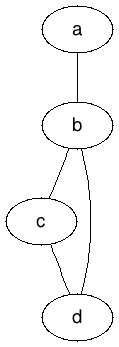
\includegraphics[width=6cm]{images/input_graph.png} 
\caption[todo]{todo}
\label{fig:arbitrary-graph}
\end{figure}

%TODO: Replace with valid nice decomposition, tag with root, and also write treewidth explicitly
\begin{figure}[here]
\centering
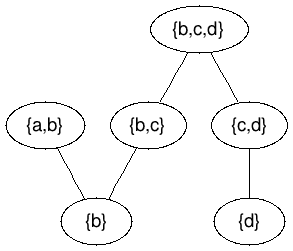
\includegraphics[width=12cm]{images/nice_tree_decomp.png} 
\caption[todo]{todo}
\label{fig:decomp-graph}
\end{figure}

\section{Counting injective homomorphisms}
As mentioned when defining the naive algorithm for countings ismorphisms, it is possible to consider maps of $P$ onto $H$, and count the number of unique such maps.
More formally we have the following:

\begin{defn}
A \emph{homomorphism} is a map $\phi : V(P) \rightarrow V(H)$ that preserves structure,
i.e. $\left\{v_1, v_2\right\} \in E(P) \Leftrightarrow \left\{\phi(v_1), \phi(v_2)\right\} \in E(H)$.
\end{defn}


An \emph{injective homomorphism} has an injective map.
%TODO: Verify runtime
%TODO: Check usage of subscript (existing homo.)
(TODO: REF Diaz) introduced an algorithm for computing the number of homorphisms $hom_{\phi}(P, H)$ in time $O^*(|H|^|P|)$.
The paper uses the terminology \emph{colorings} and requires an existing nice tree decomposition of the pattern graph, which can be computed in polynomial time in the case of bounded treewidth.

The number of isomorphic subgraphs can be evaluated by calculating the number of injective homomorphisms from $P$ to $H$, and dividing by the number of automorphisms
, i.e. $\frac{inj(P, H)}{aut(P)} = \frac{inj(P, H)}{inj(P, P)}$ (TODO: REF Fomin).

In order to retrieve partial results for the number of injective homomorphisms $inj_{\phi}(P, H)$ it is possible to apply inclusion-exlusion by a theorem due to Fomin (TODO: Ref):

\begin{thm}
%TODO: Verify runtime and add correct constraint on size of subset
Given an injective homomorphism $\phi : P \rightarrow H$ and $S \subseteq P$ then $inj_{\phi}(P \setminus S, H \setminus \phi(S))$ can be computed in time $O^*(|H|^{|P|})$.
\end{thm}

%TODO: Add description of the Fomin proof and how it uses hom() in Diaz

Hence this result can be used as a subroutine when counting the total number of injective homormophisms.

\section{Thin subgraphs as weighted disjoint triples}
Using the notions introduced up to now, it is possible to study the contributions made by (TODO: REF KASKI).

\begin{defn}
$\Delta(f, g, h) = \Sigma_{A, B, C \in S ; A \cap B = A \cap C = B \cap C = \emptyset} f(A)g(B)h(C)$
\end{defn}

Similarly to the final algorithm presented by (TODO: REF Fomin), (TODO: REF kasi) uses a partition scheme which counts all injective isomorphisms in parts.

\begin{defn}
A 3-partitioning of the pattern graph $P$ of pathwidth $p$ is a collection of pairwise disjoint sets $L \cup S \cup M \cup T \cup R = V(P)$, such that:
\begin{itemize}
\item Every edge $e \in E(P)$ connects vertices between at most two consecutive sets in the ordering $L, S, M, T, R$.
\item The separators sets have size bounded in the pathwidth, i.e. $|S|, |T| \leq p$
\item All remaining sets have $|L|, |M|, |R| \leq \frac{|P|}{3}$
\end{itemize}
\end{defn}

Now consider creating a partial injective homormophism $\phi$ mappping $S$ and $T$ onto $H$, as visualized in the following figure
, where the $A,B,C \subseteq (H \setminus \phi(S) \setminus \phi(T))$ :

\begin{figure}[here]
\centering
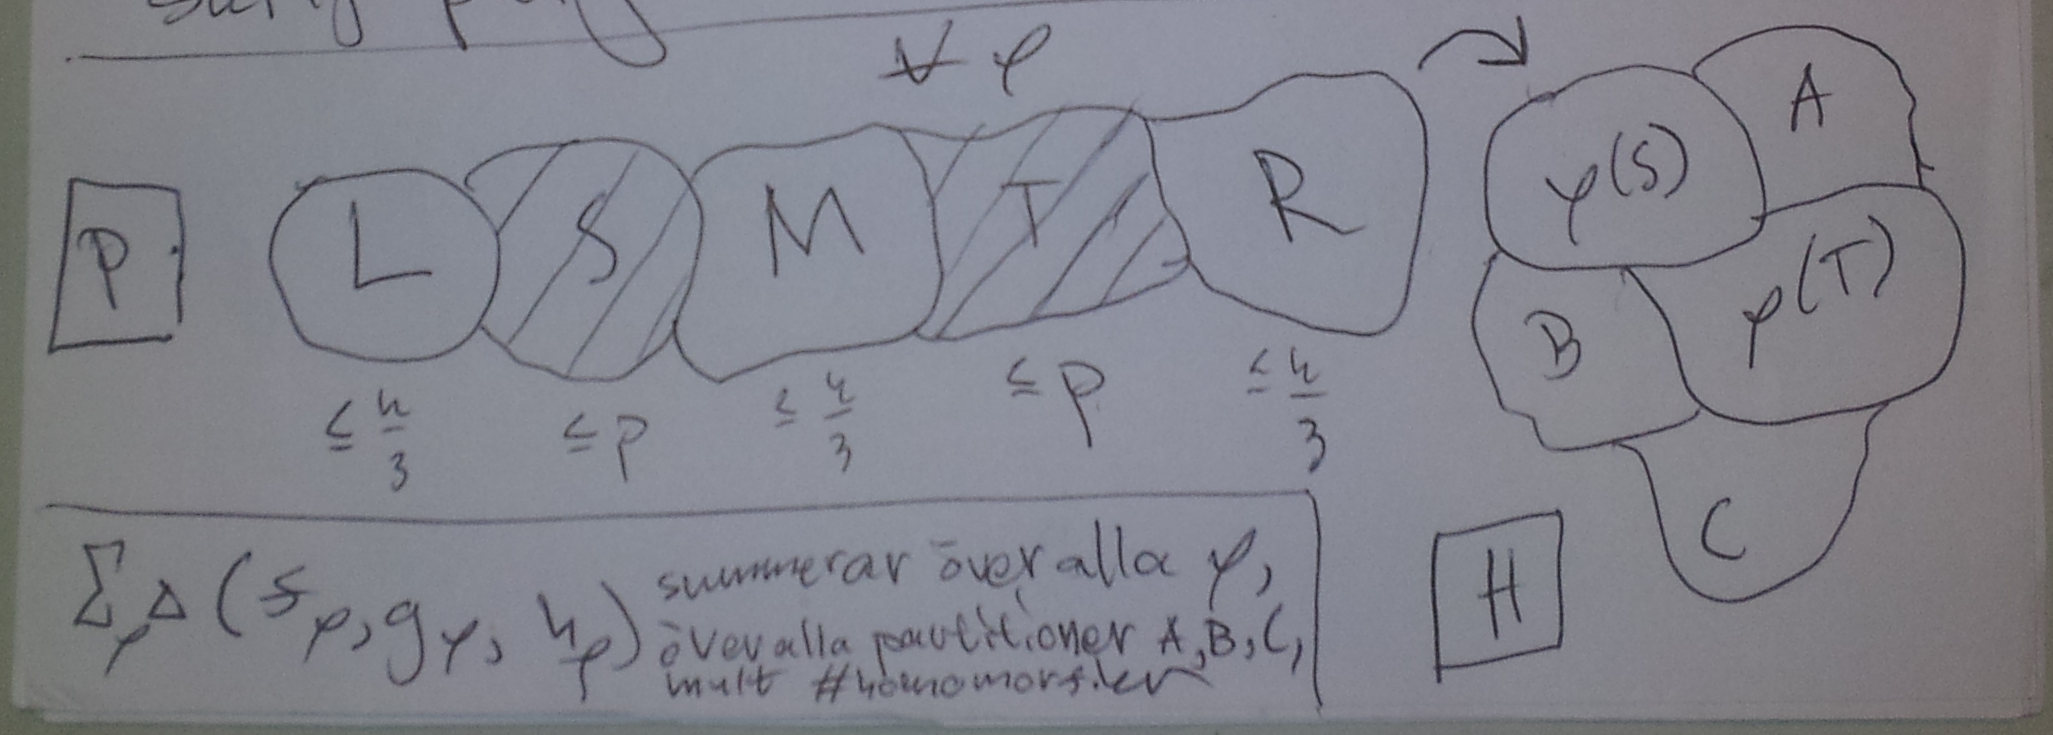
\includegraphics[width=10cm]{images/sketch_homo.png} 
\caption[todo]{todo}
\label{fig:homo-viz}
\end{figure}

Enumerating all such possible $O(|H|^{2p})$ injective homomorhpisms mapping $S$ and $T$ to the host graph,
 all possible extensions to $\phi$ can be considered using theorem TODO.
More formally the following functions over the subsets of the host graph are defined, for each candidate $\phi$:

\begin{itemize}
\item $f_\phi(A)$: The number of injective homomorphisms mapping $P[L \cup S]$ onto $H[A \cup \phi(S)]$.
\item $g_\phi(B)$: The number of injective homomorphisms mapping $P[S \cup M \cup T]$ onto $H[\phi(S) \cup B \cup \phi(T)]$.
\item $h_\phi(C)$: The number of injective homomorphisms mapping $P[R \cup T]$ onto $H[C \cup \phi(T)]$.
\end{itemize}

Hence the final number of injective homormorphisms, given a candidate $\phi$, is $\Delta_\phi(f_\phi, g_\phi, h_\phi)$.
Summing over all $\Delta_\phi$ and dividing by the number of automorphisms gives the final number of isomorphic subgraphs.

\section{Efficient weighted disjoint triples}
TODO: Kaski construction where linear system is constructed for the triples.


\chapter{Implementation}
TODO: Brief intro to this chapter

\section{General overview}
TODO: Describe implementation, trade-offs, correctness verification.

\section{Benchmarks}
TODO: Describe test data (generation and classes), scaling performance,
statistical assurance in resulsts, bottlenecks.

\section{Analysis}
TODO: analyze benchmarks

\chapter*{References}

Diaz,\\
Fomin,\\
Kaski,\\
Björklund x 2-3,\\
Flum-Grohe, \\
"An improved FPTAS for restricted shortest path" Ergun, Sinha, Zhang,\\
"Computing Bounded Path Decompositions in Logspace" Kintali, Munteanu\\
"A Linear-Time Algorithm for Finding Tree-Decompositions of Small Treewidth" Bodlaender\\
Carr, Hamish, Jack Snoeyink, and Ulrike Axen. "Computing contour trees in all dimensions." Proceedings of the eleventh annual ACM-SIAM symposium on Discrete algorithms. Society for Industrial and Applied Mathematics, 2000.\\

\end{document}
